%% Ternary complex model
%% FigInline1ThreeState.tex
%% Unused packages and definitions removed; TikZ/PGFPlots source formatted.

\documentclass{standalone}

\usepackage{tikz}
\usetikzlibrary{arrows}

\def\b{\mathsf{b}}
\def\c{\mathsf{c}}
\def\d{\mathsf{d}}

\def\kappab{\kappa_{\b}}
\def\kappac{\kappa_{\c}}

\def\etabc{\eta_{\b\c}}
\def\etacd{\eta_{\c\d}}

\def\etabc{\eta_{\b\c}}
\def\etacd{\eta_{\c\d}}

\def\kappabstar{\kappa_{\b}^*}
\def\kappacstar{\kappa_{\c}^*}

\begin{document}

\tikzset{every node/.style={minimum size=0.2cm,inner sep=2pt,outer sep=2pt}}
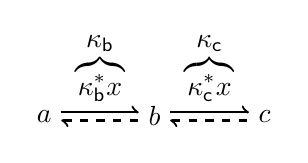
\begin{tikzpicture}[node distance=1.4cm,>=latex']
    \begin{scope}[xshift=0cm]
        \node (A) {$a$};
        \node[right of=A] (B) {$b$};
        \draw[-left to,thick,transform canvas={yshift=1.5pt}] (A) to node[above] {$\overbrace{\kappabstar x}^{\displaystyle \kappab}$} (B);
        \draw[dashed,left to-,thick,transform canvas={yshift=-1.5pt}] (A) to (B);
        \node[right of=B] (C) {$c$};
        \draw[-left to,thick,transform canvas={yshift=1.5pt}] (B) to node[above] {$\overbrace{\kappacstar x}^{\displaystyle \kappac}$} (C);
        \draw[dashed,left to-,thick,transform canvas={yshift=-1.5pt}] (B) to (C);
    \end{scope}
\end{tikzpicture}

\end{document}

